% Options for packages loaded elsewhere
\PassOptionsToPackage{unicode}{hyperref}
\PassOptionsToPackage{hyphens}{url}
\PassOptionsToPackage{dvipsnames,svgnames,x11names}{xcolor}
%
\documentclass[
  letterpaper,
  DIV=11,
  numbers=noendperiod]{scrartcl}

\usepackage{amsmath,amssymb}
\usepackage{iftex}
\ifPDFTeX
  \usepackage[T1]{fontenc}
  \usepackage[utf8]{inputenc}
  \usepackage{textcomp} % provide euro and other symbols
\else % if luatex or xetex
  \usepackage{unicode-math}
  \defaultfontfeatures{Scale=MatchLowercase}
  \defaultfontfeatures[\rmfamily]{Ligatures=TeX,Scale=1}
\fi
\usepackage{lmodern}
\ifPDFTeX\else  
    % xetex/luatex font selection
\fi
% Use upquote if available, for straight quotes in verbatim environments
\IfFileExists{upquote.sty}{\usepackage{upquote}}{}
\IfFileExists{microtype.sty}{% use microtype if available
  \usepackage[]{microtype}
  \UseMicrotypeSet[protrusion]{basicmath} % disable protrusion for tt fonts
}{}
\makeatletter
\@ifundefined{KOMAClassName}{% if non-KOMA class
  \IfFileExists{parskip.sty}{%
    \usepackage{parskip}
  }{% else
    \setlength{\parindent}{0pt}
    \setlength{\parskip}{6pt plus 2pt minus 1pt}}
}{% if KOMA class
  \KOMAoptions{parskip=half}}
\makeatother
\usepackage{xcolor}
\setlength{\emergencystretch}{3em} % prevent overfull lines
\setcounter{secnumdepth}{5}
% Make \paragraph and \subparagraph free-standing
\ifx\paragraph\undefined\else
  \let\oldparagraph\paragraph
  \renewcommand{\paragraph}[1]{\oldparagraph{#1}\mbox{}}
\fi
\ifx\subparagraph\undefined\else
  \let\oldsubparagraph\subparagraph
  \renewcommand{\subparagraph}[1]{\oldsubparagraph{#1}\mbox{}}
\fi


\providecommand{\tightlist}{%
  \setlength{\itemsep}{0pt}\setlength{\parskip}{0pt}}\usepackage{longtable,booktabs,array}
\usepackage{calc} % for calculating minipage widths
% Correct order of tables after \paragraph or \subparagraph
\usepackage{etoolbox}
\makeatletter
\patchcmd\longtable{\par}{\if@noskipsec\mbox{}\fi\par}{}{}
\makeatother
% Allow footnotes in longtable head/foot
\IfFileExists{footnotehyper.sty}{\usepackage{footnotehyper}}{\usepackage{footnote}}
\makesavenoteenv{longtable}
\usepackage{graphicx}
\makeatletter
\def\maxwidth{\ifdim\Gin@nat@width>\linewidth\linewidth\else\Gin@nat@width\fi}
\def\maxheight{\ifdim\Gin@nat@height>\textheight\textheight\else\Gin@nat@height\fi}
\makeatother
% Scale images if necessary, so that they will not overflow the page
% margins by default, and it is still possible to overwrite the defaults
% using explicit options in \includegraphics[width, height, ...]{}
\setkeys{Gin}{width=\maxwidth,height=\maxheight,keepaspectratio}
% Set default figure placement to htbp
\makeatletter
\def\fps@figure{htbp}
\makeatother

\KOMAoption{captions}{tableheading}
\makeatletter
\makeatother
\makeatletter
\makeatother
\makeatletter
\@ifpackageloaded{caption}{}{\usepackage{caption}}
\AtBeginDocument{%
\ifdefined\contentsname
  \renewcommand*\contentsname{Table of contents}
\else
  \newcommand\contentsname{Table of contents}
\fi
\ifdefined\listfigurename
  \renewcommand*\listfigurename{List of Figures}
\else
  \newcommand\listfigurename{List of Figures}
\fi
\ifdefined\listtablename
  \renewcommand*\listtablename{List of Tables}
\else
  \newcommand\listtablename{List of Tables}
\fi
\ifdefined\figurename
  \renewcommand*\figurename{Figure}
\else
  \newcommand\figurename{Figure}
\fi
\ifdefined\tablename
  \renewcommand*\tablename{Table}
\else
  \newcommand\tablename{Table}
\fi
}
\@ifpackageloaded{float}{}{\usepackage{float}}
\floatstyle{ruled}
\@ifundefined{c@chapter}{\newfloat{codelisting}{h}{lop}}{\newfloat{codelisting}{h}{lop}[chapter]}
\floatname{codelisting}{Listing}
\newcommand*\listoflistings{\listof{codelisting}{List of Listings}}
\makeatother
\makeatletter
\@ifpackageloaded{caption}{}{\usepackage{caption}}
\@ifpackageloaded{subcaption}{}{\usepackage{subcaption}}
\makeatother
\makeatletter
\@ifpackageloaded{tcolorbox}{}{\usepackage[skins,breakable]{tcolorbox}}
\makeatother
\makeatletter
\@ifundefined{shadecolor}{\definecolor{shadecolor}{rgb}{.97, .97, .97}}
\makeatother
\makeatletter
\makeatother
\makeatletter
\makeatother
\ifLuaTeX
  \usepackage{selnolig}  % disable illegal ligatures
\fi
\IfFileExists{bookmark.sty}{\usepackage{bookmark}}{\usepackage{hyperref}}
\IfFileExists{xurl.sty}{\usepackage{xurl}}{} % add URL line breaks if available
\urlstyle{same} % disable monospaced font for URLs
\hypersetup{
  pdftitle={R Installation},
  pdfauthor={Johan S. Sáenz},
  colorlinks=true,
  linkcolor={blue},
  filecolor={Maroon},
  citecolor={Blue},
  urlcolor={Blue},
  pdfcreator={LaTeX via pandoc}}

\title{R Installation}
\author{Johan S. Sáenz}
\date{2023-04-30}

\begin{document}
\maketitle
\ifdefined\Shaded\renewenvironment{Shaded}{\begin{tcolorbox}[breakable, borderline west={3pt}{0pt}{shadecolor}, boxrule=0pt, interior hidden, enhanced, frame hidden, sharp corners]}{\end{tcolorbox}}\fi

\renewcommand*\contentsname{Table of contents}
{
\hypersetup{linkcolor=}
\setcounter{tocdepth}{3}
\tableofcontents
}
\hypertarget{what-is-r}{%
\section{\texorpdfstring{\textbf{What is
R?}}{What is R?}}\label{what-is-r}}

R is a free programming language and software environment that is
broadly use for data wrangling, statistical computing and graphical
representation. It can be run on a wide variety of UNIX platforms,
Windows and MacOS.

\href{https://www.r-project.org}{The R project} is a collaborative
effort between the R developers and its community. Every R user can
develop its own packages to run in the R environment and solve different
problems or necessities. R is quite powerful but it can be challenging
to use. Because of that we used
\href{https://posit.co/download/rstudio-desktop/}{R-studio}, which is an
integrated development environment (IDE). This IDE includes a console,
syntax-highlighting editor that supports direct code execution, and
tools for plotting, history, debugging, and workspace management.

Please follow the following guide to install R and R-studio.

\hypertarget{installing-r}{%
\subsection{Installing R}\label{installing-r}}

\begin{enumerate}
\def\labelenumi{\arabic{enumi}.}
\tightlist
\item
  Go to \href{https://www.r-project.org}{The R project} website and
  click on download R.
\end{enumerate}

\begin{figure}[H]

{\centering 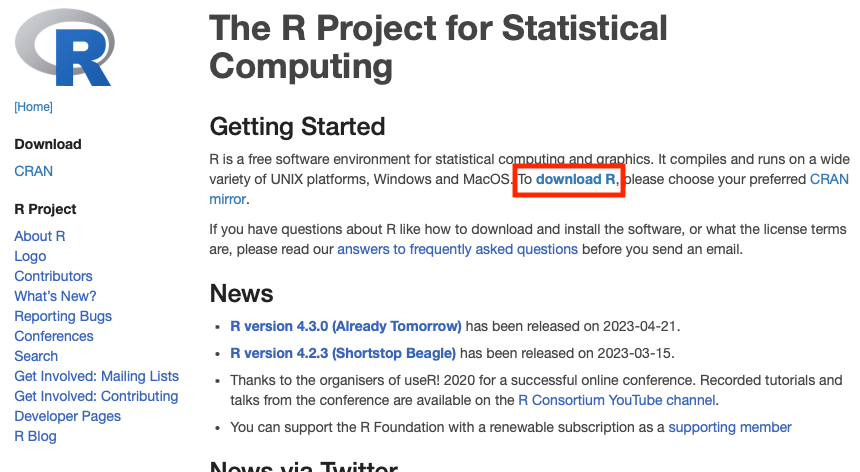
\includegraphics[width=6.77083in,height=\textheight]{FIG1.png}

}

\end{figure}

\begin{enumerate}
\def\labelenumi{\arabic{enumi}.}
\setcounter{enumi}{1}
\tightlist
\item
  Next, select a repository that is preferably located in the country
  that you are currently residing.
\end{enumerate}

\begin{figure}[H]

{\centering 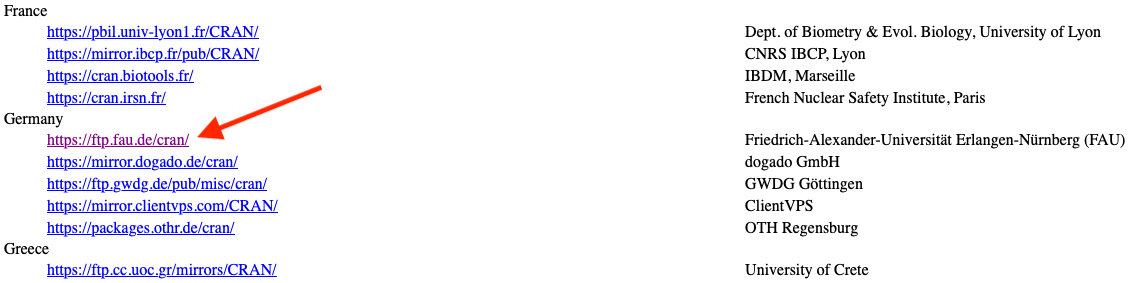
\includegraphics[width=6.77083in,height=\textheight]{FIG2.png}

}

\end{figure}

\begin{enumerate}
\def\labelenumi{\arabic{enumi}.}
\setcounter{enumi}{2}
\tightlist
\item
  After, select the the operating system (OS) that you have in your
  machine. For the following example, I will show the steps for the
  windows OS, however the instructions for the other OS are quite
  similar.
\end{enumerate}

\begin{figure}[H]

{\centering 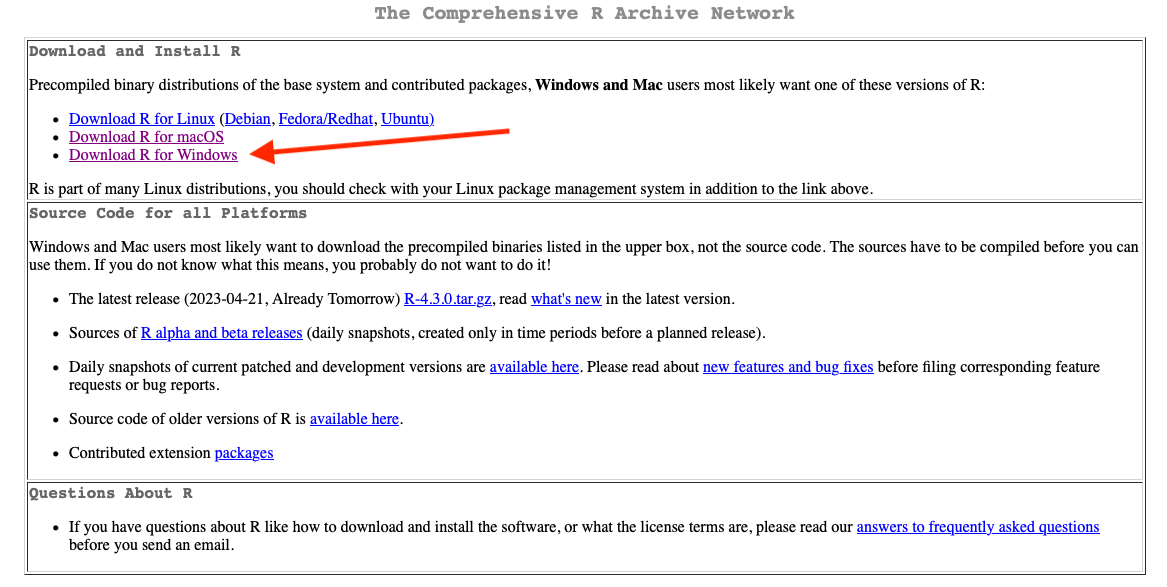
\includegraphics[width=6.77083in,height=\textheight]{Fig3.png}

}

\end{figure}

\begin{enumerate}
\def\labelenumi{\arabic{enumi}.}
\setcounter{enumi}{3}
\tightlist
\item
  Here you can click on ``install R for the first time'' or ``base''.
\end{enumerate}

\begin{figure}[H]

{\centering 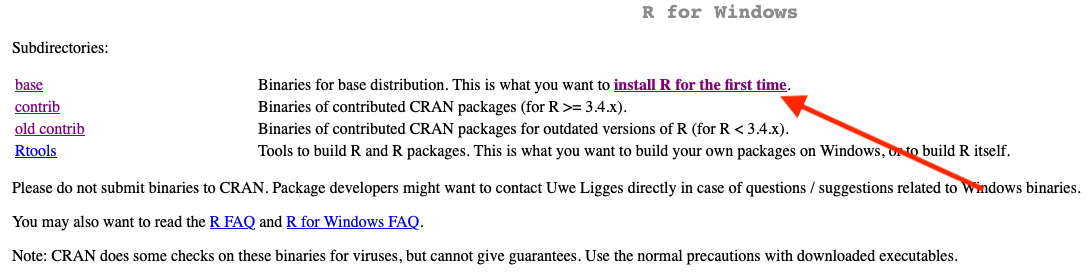
\includegraphics[width=6.77083in,height=\textheight]{fig4.png}

}

\end{figure}

\begin{enumerate}
\def\labelenumi{\arabic{enumi}.}
\setcounter{enumi}{4}
\tightlist
\item
  I usually do not install the last version available, in this case
  R-4.3.0. I prefer to to install a previous version, which would not
  have compatibility issues with some of the libraries or packages that
  I currently use. Go and click on ``Previous releases''
\end{enumerate}

\begin{figure}[H]

{\centering 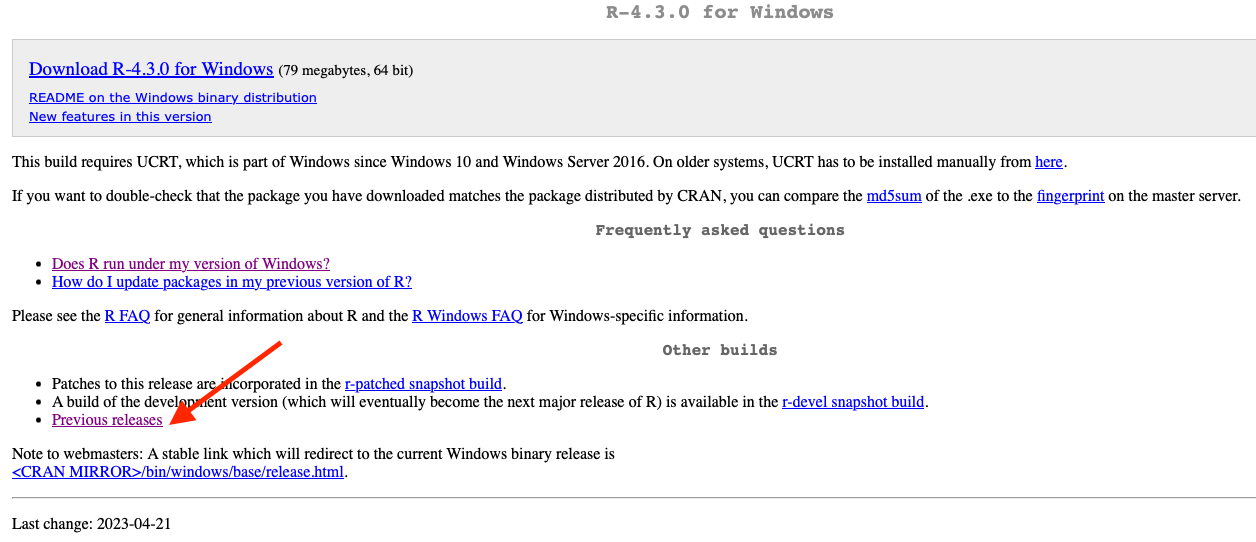
\includegraphics[width=6.77083in,height=\textheight]{fig5.png}

}

\end{figure}

\begin{enumerate}
\def\labelenumi{\arabic{enumi}.}
\setcounter{enumi}{5}
\tightlist
\item
  Select the version R-4-2.2, which have been stable during the last
  year. Go ahead and download the .exe file and install it. After,
  follow the basic installation. \textbf{I recommend you to install R in
  English not in German}. If you are in a MacOS machine be aware that
  there are different versions for the intel-based Macs and arm-based
  macs.
\end{enumerate}

\begin{figure}[H]

{\centering 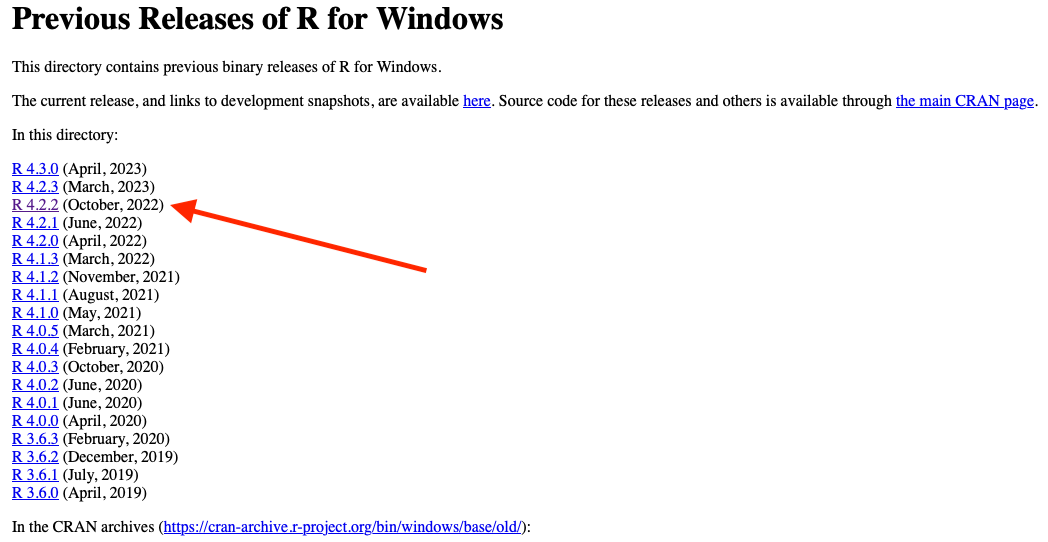
\includegraphics[width=6.77083in,height=\textheight]{Fig6.png}

}

\end{figure}

\hypertarget{r-studio-installation}{%
\subsection{R-studio installation}\label{r-studio-installation}}

\begin{enumerate}
\def\labelenumi{\arabic{enumi}.}
\tightlist
\item
  After a successful R installation, we need to install the RStudio IDE.
  Go to \href{https://posit.co/download/rstudio-desktop/}{R-studio}
  website and click on ``Donwlad RStudio desktop''. You can download the
  last version available of RStuio, follow the basic installation.
  \textbf{I recommend you to install RStudio in English not in German}.
\end{enumerate}

\begin{figure}[H]

{\centering 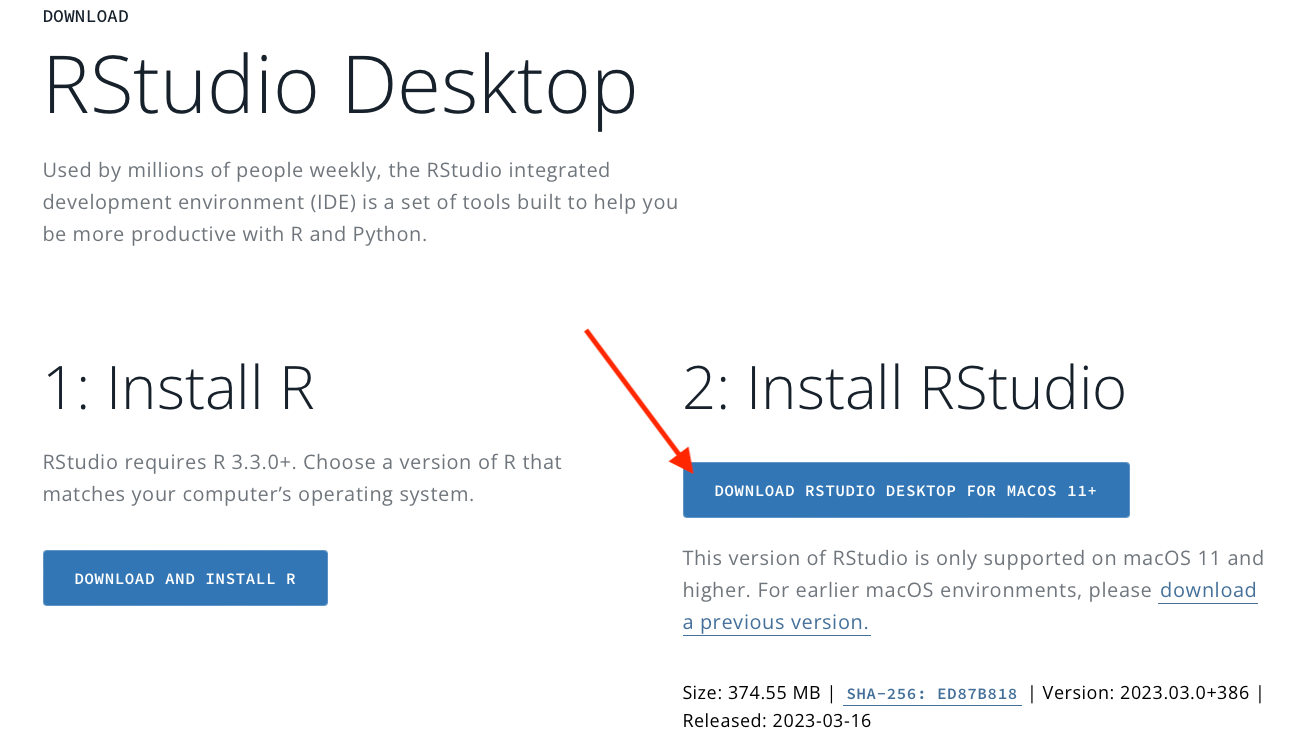
\includegraphics[width=6.77083in,height=\textheight]{fig7.png}

}

\end{figure}

\begin{enumerate}
\def\labelenumi{\arabic{enumi}.}
\setcounter{enumi}{1}
\tightlist
\item
  Finally, open RStudio and check in the console that the correct
  version of R is running under the hood.
\end{enumerate}

Now Enjoy!!!!!!!!! 😀

\begin{figure}[H]

{\centering 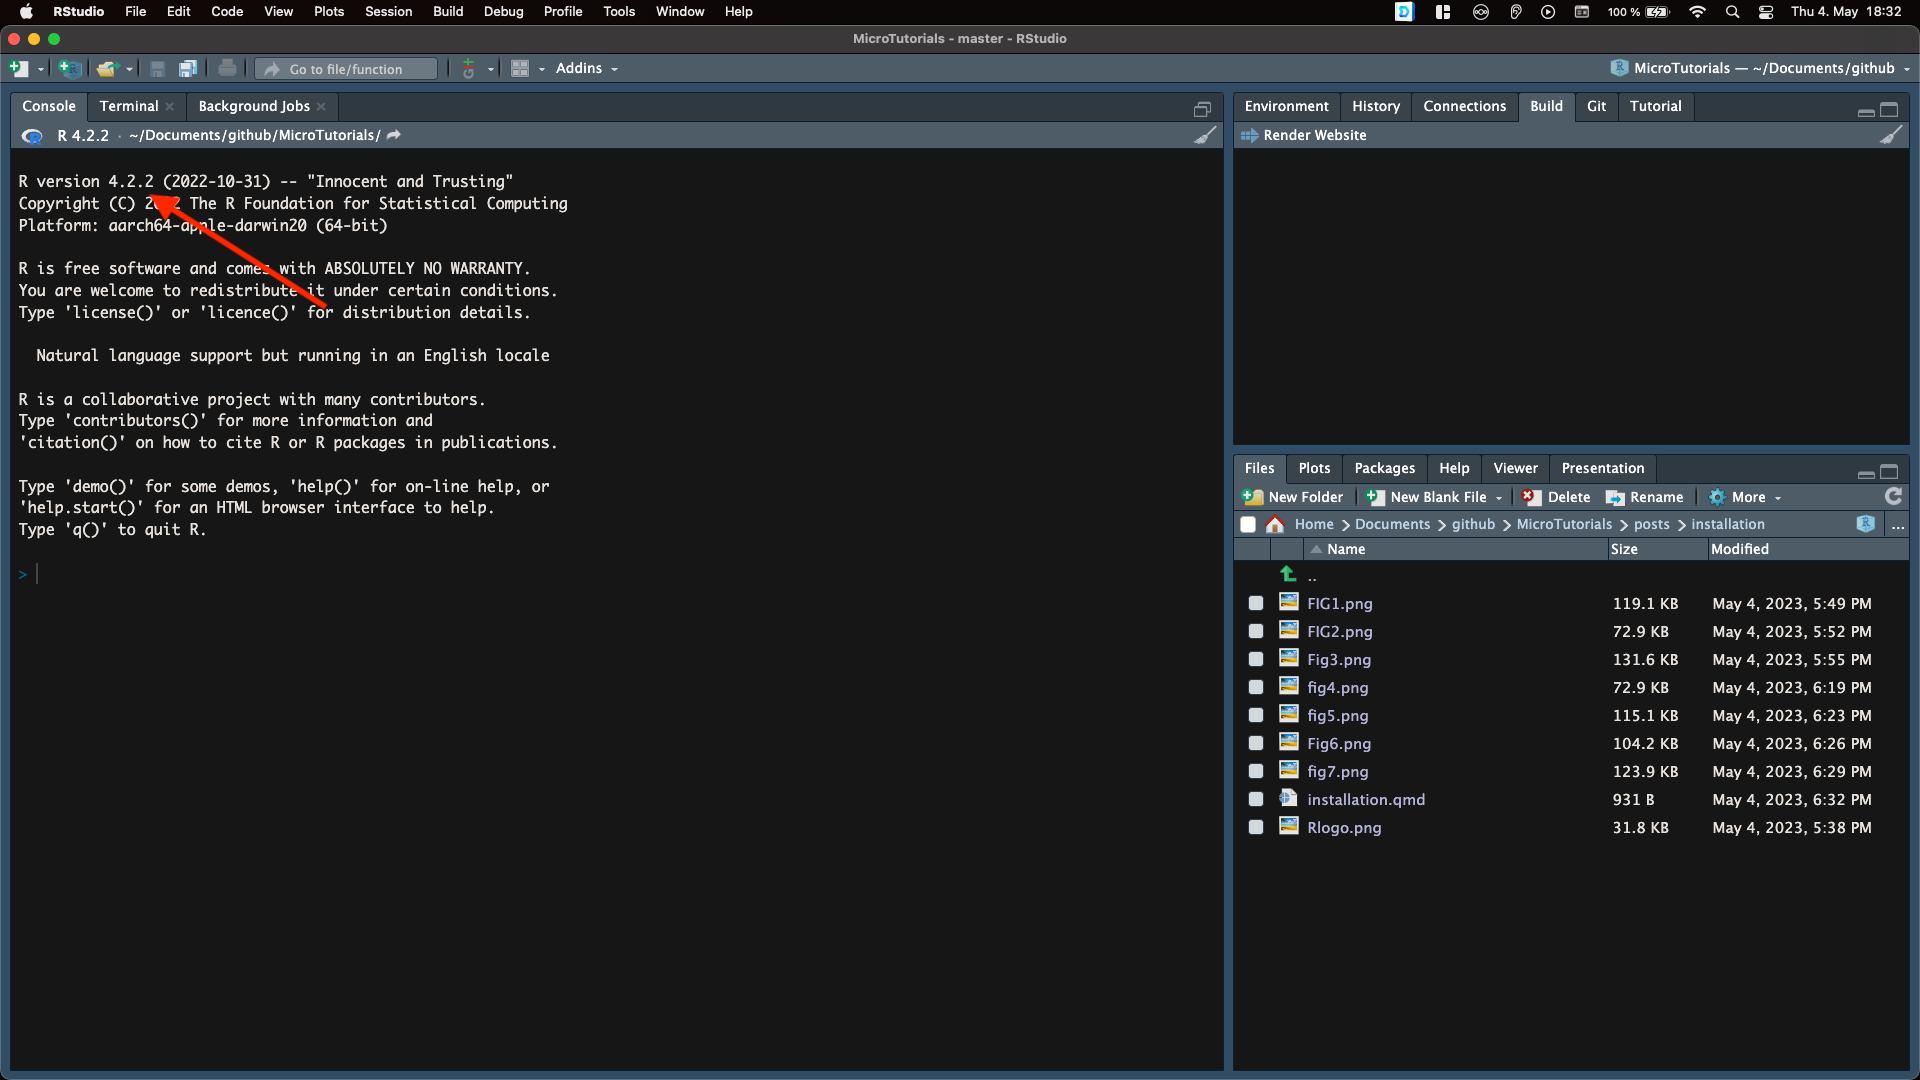
\includegraphics[width=6.77083in,height=\textheight]{Fig8.png}

}

\end{figure}



\end{document}
